\documentclass[12pt]{article}
\usepackage{amsmath}
\usepackage{amsthm}
\usepackage{amsfonts}
\usepackage{amssymb}
\usepackage{enumerate}
\usepackage{tikz}
\usepackage{pgfplots}
\pgfplotsset{compat=1.18}
\usepgfplotslibrary{fillbetween}
\usepackage[margin = .75in]{geometry}
\definecolor{purple}{RGB}{51,0,111} % Official UW color scheme
\usepackage[colorlinks=true, allcolors=purple]{hyperref} %% For links
\pagestyle{empty} %% Gets rid of the page number
%% New Commands
%% For our common number systems.
\newcommand{\Nn}{\mathbb{N}}
\newcommand{\Zz}{\mathbb{Z}}
\newcommand{\Qq}{\mathbb{Q}}
\newcommand{\Rr}{\mathbb{R}}
\newcommand\set[1]{\{ #1 \}} %%\set{abc} ==> {abc}
\newcommand\abs[1]{\left| #1 \right|} %% \abs{abc} ==> |abc|
\newcommand\parens[1]{\left( #1 \right)}
\newcommand\brac[1]{\left[ #1 \right]}
\newenvironment{solution}
  {\renewcommand\qedsymbol{$\blacksquare$}\begin{proof}[Solution]}
  {\end{proof}}


\begin{document}
\raggedright
\begin{center}
      {\large Math 1512 Calculus 1 Review: Selected Solutions}\\
  {Fall 2026}\\

\end{center}

One worked problem from each topic. Problem numbers match the review sheet, and each problem is restated before its solution.


\begin{enumerate}
\item[1.] Formulas to know.
\begin{enumerate}
\item[(c)] Give both parts of the Fundamental Theorem of Calculus.
\begin{solution}
Let $f$ be continuous on $[a,b]$.

Part 1. If $g(x) = \int_a^x f(t)\,dt$, then $g'(x) = f(x)$. The rate the area grows is the height of the graph at the moving edge.

Part 2. If $F$ is any antiderivative of $f$, meaning $F' = f$, then $\int_a^b f(x)\,dx = F(b) - F(a)$. Adding up tiny changes in $F$ gives the total change in $F$.
\end{solution}
\end{enumerate}
\item[2.] Limits from a graph.
\begin{enumerate}
\item[(b)] At which $x$ values in $(-3,4)$ is $g$ not continuous? Classify each discontinuity. At which of these is $g$ continuous from the left, or from the right?
\begin{solution}
$g$ is not continuous at $x=-1$, $0$, $2$.

At $x=-1$ the one-sided limits are $3$ and $4$: a jump. At $x=0$ the limit exists ($=1$) but is not $g(0)=3$: removable, since redefining one point fixes it. At $x=2$ the right-hand limit is infinite: an infinite discontinuity.

Continuous from the left at $a$ means $\lim_{x\to a^-} g(x) = g(a)$. This holds only at $x=2$, where both equal $1$. No point is continuous from the right: at $-1$ we compare $4$ with $1$, at $0$ we compare $1$ with $3$, and at $2$ the right limit is infinite.
\end{solution}
\end{enumerate}
\item[3.] Computing limits.
\begin{enumerate}
\item[(c)] Evaluate $\lim_{x \to -1} \frac{\frac{1}{x+3} - \frac{1}{2}}{x+1}$.
\begin{solution}
Combine the fractions in the numerator over the common denominator $2(x+3)$.

\[\frac{1}{x+1}\cdot\frac{2-(x+3)}{2(x+3)} = \frac{1}{x+1}\cdot\frac{-(x+1)}{2(x+3)} = \frac{-1}{2(x+3)} \longrightarrow -\frac14.\]
\end{solution}
\end{enumerate}
\item[4.] Squeeze Theorem.
\begin{enumerate}
\item[(a)] Evaluate $\lim_{x \to 0} x^2 \sin\parens{\frac{3}{x}}$.
\begin{solution}
$\sin\parens{\frac{3}{x}}$ oscillates and has no limit, so the product law does not apply (this answers (c)). But it is bounded: $-1 \le \sin\parens{\frac3x} \le 1$. Multiplying by $x^2 \ge 0$,

\[-x^2 \le x^2 \sin\parens{\frac{3}{x}} \le x^2.\]

Both bounds go to $0$, so by the Squeeze Theorem the limit is $0$. The $x^2$ crushes the oscillation.
\end{solution}
\end{enumerate}
\item[5.] Limits at infinity.
\begin{enumerate}
\item[(a)] Evaluate $\lim_{x \to -\infty} \frac{\sqrt{4x^2+1}}{x+3}$.
\begin{solution}
Pull $x^2$ out of the root: $\sqrt{4x^2+1} = \sqrt{x^2}\sqrt{4+\frac{1}{x^2}} = \abs{x}\sqrt{4+\frac{1}{x^2}}$. For $x<0$, $\abs{x} = -x$.

\[\frac{-x\sqrt{4+\frac{1}{x^2}}}{x\parens{1+\frac{3}{x}}} = \frac{-\sqrt{4+\frac{1}{x^2}}}{1+\frac{3}{x}} \longrightarrow -2.\]

The sign makes sense: the top is positive and the bottom is negative for very negative $x$.
\end{solution}
\end{enumerate}
\item[6.] Continuity and the IVT.
\begin{enumerate}
\item[(b)] Find $a$ and $b$ so that $f(x) = \begin{cases} 2 & x < 1 \\ ax + b & 1 \leq x < 4 \\ 8 & x \geq 4 \end{cases}$ is continuous everywhere.
\begin{solution}
Each piece is continuous, so only the seams at $x=1$ and $x=4$ matter. The middle line must start at height $2$ and end at height $8$.

\[a + b = 2, \qquad 4a + b = 8.\]

Subtracting, $3a = 6$, so $a = 2$ and $b = 0$. The middle piece is $2x$.
\end{solution}
\end{enumerate}
\item[7.] The derivative as a limit.
\begin{enumerate}
\item[(b)] Compute $f'(x)$ directly from $f'(x) = \lim_{h \to 0} \frac{f(x+h)-f(x)}{h}$ for $f(x) = \frac{x}{x+2}$.
\begin{solution}
Combine the fractions in the numerator first.

\[\frac{1}{h}\parens{\frac{x+h}{x+h+2}-\frac{x}{x+2}} = \frac{(x+h)(x+2) - x(x+h+2)}{h(x+h+2)(x+2)} = \frac{2h}{h(x+h+2)(x+2)}.\]

Cancel $h$ and let $h\to0$: $f'(x) = \frac{2}{(x+2)^2}$.
\end{solution}
\end{enumerate}
\item[8.] Differentiation rules.
\begin{enumerate}
\item[(b)] Find the points on the curve $y = x^3 - 3x^2 - 9x + 2$ where the tangent line is parallel to the line $y = 15x$.
\begin{solution}
Parallel lines have equal slopes, so we need $y' = 15$.

\[3x^2 - 6x - 9 = 15 \quad\Longrightarrow\quad x^2 - 2x - 8 = 0 \quad\Longrightarrow\quad (x-4)(x+2) = 0.\]

At $x = 4$, $y = 64 - 48 - 36 + 2 = -18$, and at $x=-2$, $y = -8 - 12 + 18 + 2 = 0$. The points are $(4,-18)$ and $(-2,0)$.
\end{solution}
\end{enumerate}
\item[9.] Trig derivatives.
\begin{enumerate}
\item[(b)] Evaluate $\lim_{x \to 0} \frac{\sin(4x)}{3x}$ and $\lim_{x \to 0} \frac{1-\cos x}{x\sin x}$.
\begin{solution}
\[\frac{\sin(4x)}{3x} = \frac43\cdot\frac{\sin(4x)}{4x} \longrightarrow \frac43.\]

For the second, multiply by $\frac{1+\cos x}{1+\cos x}$ and use $1-\cos^2 x = \sin^2 x$.

\[\frac{1-\cos^2 x}{x\sin x\,(1+\cos x)} = \frac{\sin^2 x}{x\sin x\,(1+\cos x)} = \frac{\sin x}{x}\cdot\frac{1}{1+\cos x} \longrightarrow 1\cdot\frac12 = \frac12.\]
\end{solution}
\end{enumerate}
\item[10.] Chain rule.
\begin{enumerate}
\item[(a)] Use the table to find $(f \circ g)'(1)$, $(g \circ f)'(1)$, and $(fg)'(2)$. $$\begin{array}{c|cccc} x & 0 & 1 & 2 & 3 \\ \hline f(x) & 2 & 3 & 0 & 1 \\ f'(x) & -1 & 4 & 2 & 5 \\ g(x) & 1 & 2 & 3 & 0 \\ g'(x) & 3 & -2 & 1 & 4 \end{array}$$
\begin{solution}
The chain rule evaluates the outer derivative at the inner value: $(f\circ g)'(1) = f'(g(1))\,g'(1) = f'(2)\cdot(-2) = 2(-2) = -4$.

$(g\circ f)'(1) = g'(f(1))\,f'(1) = g'(3)\cdot 4 = 16$.

The product rule gives $(fg)'(2) = f'(2)g(2) + f(2)g'(2) = 2\cdot3 + 0\cdot1 = 6$.
\end{solution}
\end{enumerate}
\item[11.] Implicit differentiation.
\begin{enumerate}
\item[(b)] Find the tangent line to $\sin(x+y) = 2x - 2y$ at $(\pi, \pi)$.
\begin{solution}
Check the point: $\sin(2\pi) = 0 = 2\pi - 2\pi$. Differentiate.

\[\cos(x+y)\,(1+y') = 2 - 2y'.\]

At the point $\cos(2\pi) = 1$, so $1 + y' = 2 - 2y'$ and $y' = \frac13$. The tangent line is $y = \pi + \frac13(x-\pi)$.
\end{solution}
\end{enumerate}
\item[12.] Related rates.
\begin{enumerate}
\item[(b)] A tank is an inverted cone with radius 3 m at the top and height 6 m. Water is pumped in at 4 $\text{m}^3$/min. How fast is the water level rising when the water is 4 m deep?
\begin{solution}
Let $h$ be the depth and $r$ the radius of the water surface. Similar triangles give $\frac{r}{h} = \frac36$, so $r = \frac h2$ and

\[V = \frac13\pi r^2 h = \frac{\pi h^3}{12}, \qquad \frac{dV}{dt} = \frac{\pi h^2}{4}\frac{dh}{dt}.\]

At $h=4$: $4 = 4\pi \frac{dh}{dt}$, so $\frac{dh}{dt} = \frac{1}{\pi}$ m/min. The factor $\frac{\pi h^2}{4}$ is the area of the water surface, which is why the level rises more slowly as the tank fills.
\end{solution}
\end{enumerate}
\item[13.] Linear approximation.
\begin{enumerate}
\item[(a)] Find the linearization of $f(x) = \sqrt[3]{x}$ at $a=27$. Use it to approximate $\sqrt[3]{27.27}$.
\begin{solution}
$f(27) = 3$ and $f'(x) = \frac13 x^{-2/3}$, so $f'(27) = \frac{1}{27}$. Then $L(x) = 3 + \frac{x-27}{27}$ and $L(27.27) = 3 + \frac{0.27}{27} = 3.01$. The true value is $3.00997\ldots$
\end{solution}
\end{enumerate}
\item[14.] Extreme values.
\begin{enumerate}
\item[(c)] Find the absolute max and min of $f(x) = x\sqrt{4-x^2}$ on $[-1,2]$.
\begin{solution}
By the product and chain rules,

\[f'(x) = \sqrt{4-x^2} - \frac{x^2}{\sqrt{4-x^2}} = \frac{4 - 2x^2}{\sqrt{4-x^2}}.\]

$f' = 0$ at $x = \pm\sqrt2$, and only $\sqrt2$ is in $[-1,2]$. $f'$ is undefined at $x = 2$, an endpoint anyway.

$f(-1) = -\sqrt3$, $f(\sqrt2) = \sqrt2\cdot\sqrt2 = 2$, $f(2) = 0$. Max $2$ at $x = \sqrt2$, min $-\sqrt3$ at $x = -1$.
\end{solution}
\end{enumerate}
\item[15.] Mean Value Theorem.
\begin{enumerate}
\item[(c)] Show that $x^3 + 5x - 2 = 0$ has exactly one real solution.
\begin{solution}
Let $f(x) = x^3 + 5x - 2$. At least one: $f(0) = -2 < 0 < 4 = f(1)$, so the IVT gives a root in $(0,1)$.

At most one: if $f(a) = f(b) = 0$ with $a<b$, the MVT gives $c$ with $f'(c) = \frac{0-0}{b-a} = 0$. But $f'(x) = 3x^2 + 5 \ge 5$. So a second root is impossible.
\end{solution}
\end{enumerate}
\item[16.] Shape of a graph.
\begin{enumerate}
\item[(a)] For $f(x) = x^3 - 6x^2 + 9x + 1$, find the intervals of increase and decrease, local extrema, concavity, and inflection points.
\begin{solution}
$f'(x) = 3x^2 - 12x + 9 = 3(x-1)(x-3)$. So $f' > 0$ on $(-\infty,1)$ and $(3,\infty)$ (increasing) and $f'<0$ on $(1,3)$ (decreasing).

$f'$ changes from $+$ to $-$ at $1$: local max $f(1) = 5$. From $-$ to $+$ at $3$: local min $f(3) = 1$.

$f''(x) = 6x - 12$: concave down on $(-\infty,2)$, concave up on $(2,\infty)$, inflection point $(2,3)$. The inflection point sits halfway between the max and min, as for every cubic.
\end{solution}
\end{enumerate}
\item[17.] Curve sketching.
\begin{enumerate}
\item[(b)] Sketch $f(x) = \frac{x^2}{x-1}$, labeling all key features.
\begin{solution}
Domain $x \ne 1$. The only intercept is $(0,0)$. At $x=1$ the top is $1 \ne 0$, so $x = 1$ is a vertical asymptote: $f\to-\infty$ as $x\to1^-$ and $f\to\infty$ as $x\to1^+$.

There is no horizontal asymptote, since the top has higher degree. Long division gives $\frac{x^2}{x-1} = x + 1 + \frac{1}{x-1}$, and $\frac{1}{x-1}\to0$, so the graph approaches the slant asymptote $y = x+1$ as $x \to \pm\infty$.

\[f'(x) = \frac{x(x-2)}{(x-1)^2}, \qquad f''(x) = \frac{2}{(x-1)^3}.\]

Increasing on $(-\infty,0)$ and $(2,\infty)$, decreasing on $(0,1)$ and $(1,2)$. Local max $(0,0)$, local min $(2,4)$. Concave down on $(-\infty,1)$, concave up on $(1,\infty)$, no inflection point. The graph is two branches hugging $y = x+1$, one with a peak at the origin and one with a valley at $(2,4)$.
\end{solution}
\end{enumerate}
\item[18.] Optimization.
\begin{enumerate}
\item[(b)] A closed cylindrical can holds $16\pi\ \text{cm}^3$. Find the radius and height that minimize its surface area.
\begin{solution}
$\pi r^2 h = 16\pi$, so $h = \frac{16}{r^2}$. The surface area is two disks plus the side.

\[S(r) = 2\pi r^2 + 2\pi r h = 2\pi r^2 + \frac{32\pi}{r}, \qquad S'(r) = 4\pi r - \frac{32\pi}{r^2}.\]

$S' = 0$ gives $r^3 = 8$, so $r = 2$ cm and $h = 4$ cm. $S'' > 0$ for $r>0$, so this is a min. The best can has height equal to its diameter.
\end{solution}
\end{enumerate}
\item[19.] Antiderivatives.
\begin{enumerate}
\item[(c)] A particle has $a(t) = 6t - 4$, $v(0) = 3$, $s(0) = 1$. Find $s(t)$.
\begin{solution}
$v(t) = 3t^2 - 4t + 3$ (the constant is $v(0)$), and $s(t) = t^3 - 2t^2 + 3t + 1$ (the constant is $s(0)$).
\end{solution}
\end{enumerate}
\item[20.] Riemann sums.
\begin{enumerate}
\item[(c)] Write $\lim_{n \to \infty} \sum_{i=1}^n \frac{3}{n}\sqrt{1 + \frac{3i}{n}}$ as a definite integral, then evaluate it.
\begin{solution}
Read $\Delta x = \frac3n$ and $x_i = 1 + \frac{3i}{n}$, so the interval starts at $1$ and has length $3$, and the height is $\sqrt{x_i}$.

\[\int_1^4 \sqrt{x}\,dx = \frac23\brac{x^{3/2}}_1^4 = \frac23(8-1) = \frac{14}{3}.\]
\end{solution}
\end{enumerate}
\item[21.] The integral as area.
\begin{enumerate}
\item[(d)] For the velocity graph below ($v$ in m/s, $t$ in s), find the displacement and total distance from $t=0$ to $t=10$, the position at $t=10$ if $x(0)=3$ m, the acceleration at $t=5$, and when the particle is farthest from its start.
\begin{center}
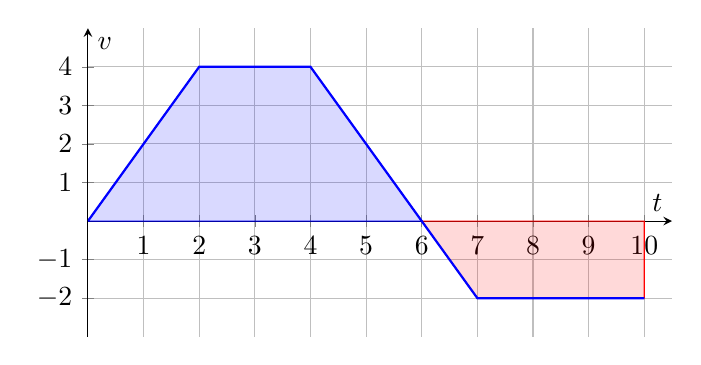
\begin{tikzpicture}
\begin{axis}[width=9cm, height=5.5cm, xmin=0, xmax=10.5, ymin=-3, ymax=5, axis lines=middle, grid=major, xtick={0,...,10}, ytick={-2,...,4}, xlabel={$t$}, ylabel={$v$}]
    \addplot[blue, fill=blue, fill opacity=0.15] coordinates {(0,0) (2,4) (4,4) (6,0)} -- cycle;
    \addplot[red, fill=red, fill opacity=0.15] coordinates {(6,0) (7,-2) (10,-2) (10,0)} -- cycle;
    \addplot[blue, thick] coordinates {(0,0) (2,4) (4,4) (7,-2) (10,-2)};
\end{axis}
\end{tikzpicture}
\end{center}
\begin{solution}
Displacement is the signed area under $v$. Above the axis (blue): triangle $4$, rectangle $8$, triangle $4$, total $16$. Below (red): triangle $1$ and rectangle $6$, total $7$.

\[\text{displacement} = 16 - 7 = 9\ \text{m}, \qquad \text{distance} = 16 + 7 = 23\ \text{m}.\]

The position at $t = 10$ is $3 + 9 = 12$ m. The acceleration at $t=5$ is the slope of the segment from $(4,4)$ to $(7,-2)$, which is $-2\ \text{m/s}^2$.

The particle moves forward while $v>0$ and backward after $t=6$, so it is farthest from the start at $t = 6$, $16$ m away.
\end{solution}
\end{enumerate}
\item[22.] Fundamental Theorem, Part 1.
\begin{enumerate}
\item[(c)] Find $g'(x)$ if $g(x) = \int_{2x}^{x^3} \frac{1}{1+t^4} dt$.
\begin{solution}
Split at $0$ and apply FTC 1 with the chain rule to each piece.

\[g'(x) = \frac{3x^2}{1+x^{12}} - \frac{2}{1+16x^4}.\]
\end{solution}
\end{enumerate}
\item[23.] Fundamental Theorem, Part 2.
\begin{enumerate}
\item[(c)] What is wrong with $\int_{-1}^2 \frac{1}{x^2} dx = \brac{-\frac{1}{x}}_{-1}^2 = -\frac{3}{2}$?
\begin{solution}
FTC 2 needs $f$ continuous on $[a,b]$, and $\frac{1}{x^2}$ blows up at $x=0$, inside $[-1,2]$. The answer cannot be right anyway, because $\frac1{x^2} > 0$ and the integral of a positive function cannot be negative. (This integral is improper, and it diverges. Improper integrals come in Calculus 2.)
\end{solution}
\end{enumerate}
\item[24.] Substitution.
\begin{enumerate}
\item[(c)] Evaluate $\int_{-2}^1 x\sqrt{x+3}\, dx$.
\begin{solution}
Let $u = x+3$, so $du = dx$, $x = u - 3$, and the bounds become $1$ and $4$.

\[\int_1^4 (u-3)u^{1/2}\,du = \brac{\frac25u^{5/2} - 2u^{3/2}}_1^4 = \parens{\frac{64}{5} - 16} - \parens{\frac25 - 2} = -\frac85.\]

The answer is negative because $x\sqrt{x+3}$ is negative on most of $[-2,1]$.
\end{solution}
\end{enumerate}
\item[25.] Area between curves.
\begin{enumerate}
\item[(b)] Find the area between $y = \sqrt{x}$ and $y = \frac{x}{3}$, integrating with respect to $x$, then with respect to $y$.
\begin{solution}
They meet where $\sqrt x = \frac x3$: $x = 0$ and $x = 9$, at heights $0$ and $3$. The root is on top (at $x = 1$: $1 > \frac13$).

\[\int_0^9\parens{\sqrt x - \frac x3}dx = \brac{\frac23x^{3/2} - \frac{x^2}{6}}_0^9 = 18 - \frac{27}{2} = \frac92.\]

In $y$, solve each curve for $x$: the line is $x = 3y$ (on the right) and the root is $x = y^2$ (on the left).

\[\int_0^3\parens{3y - y^2}dy = \frac{27}{2} - 9 = \frac92.\]
\end{solution}
\end{enumerate}
\item[26.] Average value.
\begin{enumerate}
\item[(b)] Find the average value of $f(x) = x^2$ on $[0,3]$ and a $c$ in $[0,3]$ with $f(c)$ equal to it.
\begin{solution}
$f_{\text{ave}} = \frac13\int_0^3x^2\,dx = \frac13\cdot 9 = 3$. Then $c^2 = 3$ gives $c = \sqrt3$, which is in $[0,3]$. The Mean Value Theorem for integrals says such a $c$ always exists for continuous $f$.
\end{solution}
\end{enumerate}
\item[27.] Volumes.
\begin{enumerate}
\item[(c)] Revolve the region between $y = \sqrt{x}$ and $y = x^2$ around the $y$-axis, and then around the line $x = -1$.
\begin{solution}
They meet at $(0,0)$ and $(1,1)$. Both axes are vertical, so slice horizontally. At height $y$ the region runs from the parabola $x = y^2$ (inner) out to the root curve $x = \sqrt y$ (outer).

\[V_{y\text{-axis}} = \pi\int_0^1\parens{y - y^4}dy = \pi\parens{\frac12 - \frac15} = \frac{3\pi}{10}.\]

Around $x = -1$ each radius grows by $1$: $R = \sqrt y + 1$ and $r = y^2 + 1$.

\[V = \pi\int_0^1\parens{(\sqrt y + 1)^2 - (y^2+1)^2}dy = \pi\int_0^1\parens{y + 2\sqrt y - y^4 - 2y^2}dy = \frac{29\pi}{30}.\]
\end{solution}
\end{enumerate}
\item[28.] Work.
\begin{enumerate}
\item[(c)] A 10 m chain with mass 2 kg per meter hangs from the top of a building. How much work does it take to pull the whole chain up to the top? Use $g = 9.8\ \text{m}/\text{s}^2$.
\begin{solution}
After $x$ meters have been pulled up, $10 - x$ meters still hang, with weight $2(9.8)(10-x) = 19.6(10-x)$ N. That is the force needed to lift the next small piece $dx$.

\[W = \int_0^{10} 19.6(10-x)\,dx = 19.6\brac{10x - \frac{x^2}{2}}_0^{10} = 19.6\cdot 50 = 980\ \text{J}.\]

Check: the chain's center of mass rises $5$ m, and $(20\ \text{kg})(9.8)(5\ \text{m}) = 980$ J.
\end{solution}
\end{enumerate}
\end{enumerate}
\end{document}
